\subsection{Examples of complex EPNs}
\label{sec:CplxEPNs}

In this section, we provide examples of Entity Pool Node representations drawn using the \SBGNPDLone glyphs described above. 

\fig{example-camkii} represents a pool of calcium/calmodulin kinase II entities, each with phosphorylation on the sites threonine 286 and 306, as well as catalytic and autoinhibitory domains.  Note the use of \emph{units of information} and \emph{state variables}.

\begin{figure}[H]
  \centering
  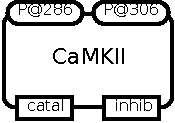
\includegraphics[scale = 0.8]{images/build/macromolecule_camkii_example.pdf}
  \caption{An example representation of calcium/calmodulin kinase II EPN.}
  \label{fig:example-camkii}
\end{figure}

\fig{example-glur} represents the glutamate receptor in the open state, with both phosphorylation and glycosylation.  The entity carries two functional domains, the ligand-binding domain and the ion pore, and its chemical nature is presided.

\begin{figure}[H]
  \centering
  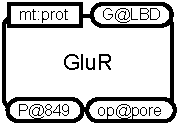
\includegraphics[scale = 0.8]{images/build/macromolecule_glu_r_example.pdf}
  \caption{An example of a glutamate receptor in the open state.}
  \label{fig:example-glur}
\end{figure}
